\documentclass[aspectratio=169]{beamer}              % only frames

% for themes, etc.
\mode<presentation>
\usetheme{Madrid} 
\usecolortheme{crane}

%\usepackage{times}  % fonts are up to you
% The usual suspects
\usepackage{multirow, booktabs, dcolumn, color, graphicx} % Tables\usepackage{graphicx}
\usepackage{amsmath,amssymb,amsthm}
% Strikethrough text
\usepackage{soul}
% Adjust box to fit tabulars
\usepackage{adjustbox}
% Embed video
\usepackage{media9}
% For notes
\usepackage{pgfpages}
%\setbeameroption{hide notes} % Only slides
%\setbeameroption{show only notes} % Only notes
\setbeameroption{show notes on second screen=right} % Both
% Give a slight yellow tint to the notes page
%\setbeamertemplate{note page}{\pagecolor{yellow!5}\insertnote}\usepackage{palatino}
% Use colors by name
\usepackage{xcolor}
% EMBEDDING VIDEO IS POSSIBLE WITH PDFPC USE PDF PC to present
\usepackage{multimedia}



% The table highlighting for hypothesis discussion.
\usepackage[beamer,customcolors]{hf-tikz}
\usetikzlibrary{calc}

% To use background images
\newenvironment{colorframe}[2][]{%
\setbeamercolor{background canvas}{bg=#1}
\begin{frame}\color{white}}
{\end{frame}}


% To set the hypothesis highlighting boxes red.
\tikzset{hl/.style={
    set fill color=red!80!black!40,
    set border color=red!80!black,
  },
}

% Set Graphics folder
\graphicspath{{./figures/}}


% these will be used later in the title page
\title{Harrasment Online}
\subtitle{How To Survive a Troll Attack}
\author{Irfan Kanat}
\institute[CBS]{{Department of Digitization}\\ Copenhagen Business School}
%\date{\today}



\begin{document}

% this prints title, author etc. info from above
\begin{frame}

	\titlepage

	\vfill
	{\tiny This work is licensed under a \href{http://creativecommons.org/licenses/by/4.0/}{Creative Commons Attribution 4.0 International License}.}

\end{frame}

\note{Oh sweet summer child, you can never return to that home of your childhood again. For you are not the same person that left...}


\begin{frame}
	\frametitle{Today's Objectives}
    
    \begin{itemize}
    	\item Abuse and Harrassment Online
    	\item Factors Leading to Exposure
    	\item How to Respond
    \end{itemize}

\end{frame}


\begin{colorframe}[black]

	\centering
	\Large
	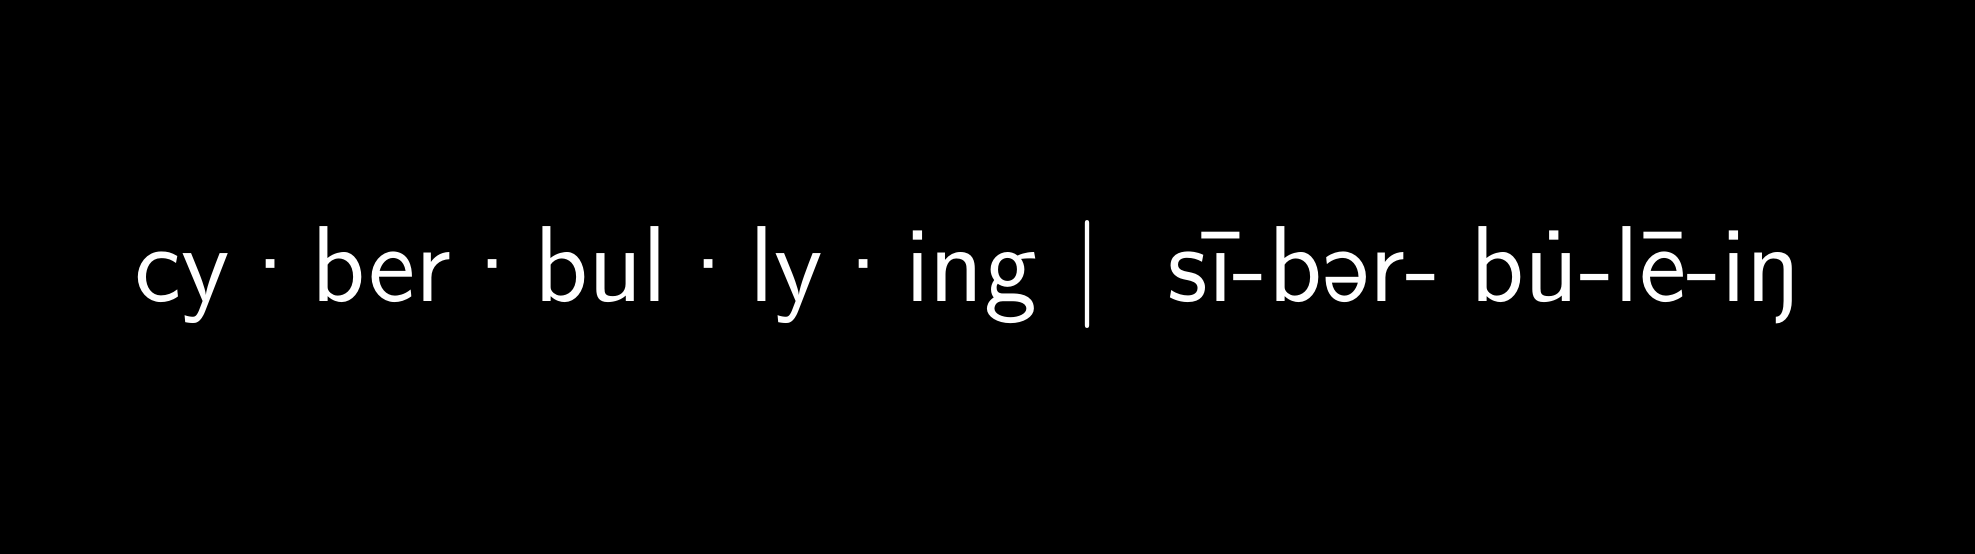
\includegraphics[width = \textwidth, height = .85\textheight, keepaspectratio]{figures/phonetics.png} 

\end{colorframe}

\note{``Cyberbullying is posting meanspirited messages online, often about a young person, often done anonymously.'' says Merriam Webster.

Cyberbullying research center defines it as ``willful and repeated harm inflicted through the use of computers, cell phones, and other electronic devices''.

It can escalate to more serious forms of harrasment if not taken care of.}

\begin{frame}
	\frametitle{Horror Stories are Real}

	    \begin{columns}
			\begin{column}{0.6\textwidth}
	
				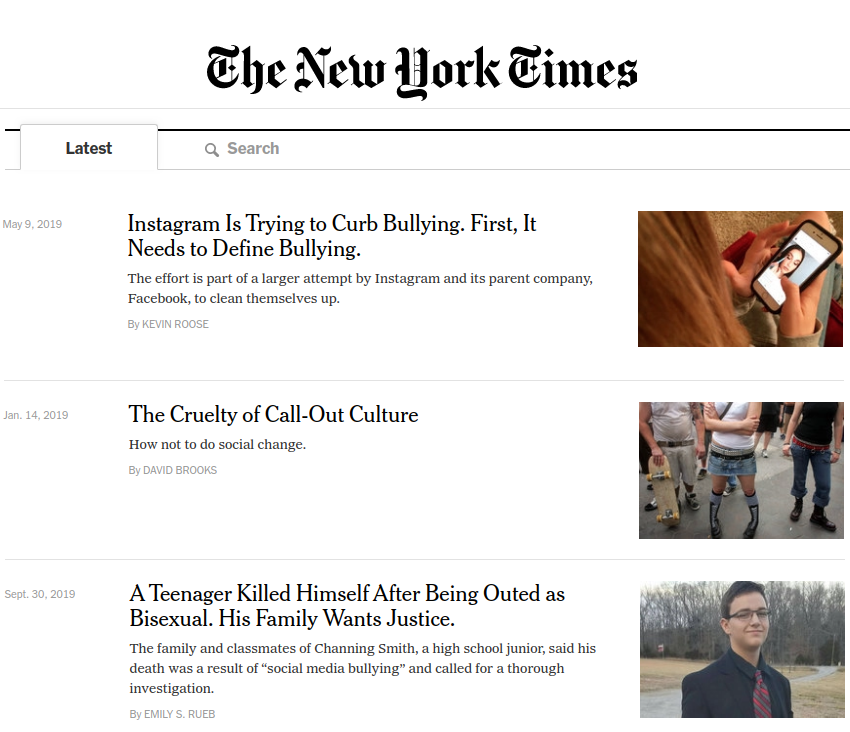
\includegraphics[width = \textwidth, height = .85\textheight, keepaspectratio]{figures/NYT.png}
		
			\end{column}
	
			\begin{column}{0.4\textwidth}
	
				Becoming a Victim is Trivial
	
			\end{column}
	
		\end{columns}



\end{frame}

\note{ It is such a common thing that NYT has a special topic tracker just for Cyberbullying.

The cost of entry for cyber bullying is truly low. In an environment defined by anonymity, throngs take courage they may not otherwise have. Fueled by a mindless herd mentality they viciously attack those who are victimized.

Unfortunately, things don't usually remain confined to mean spirited messages.}

\begin{colorframe}[black]

	\centering
	\Large
	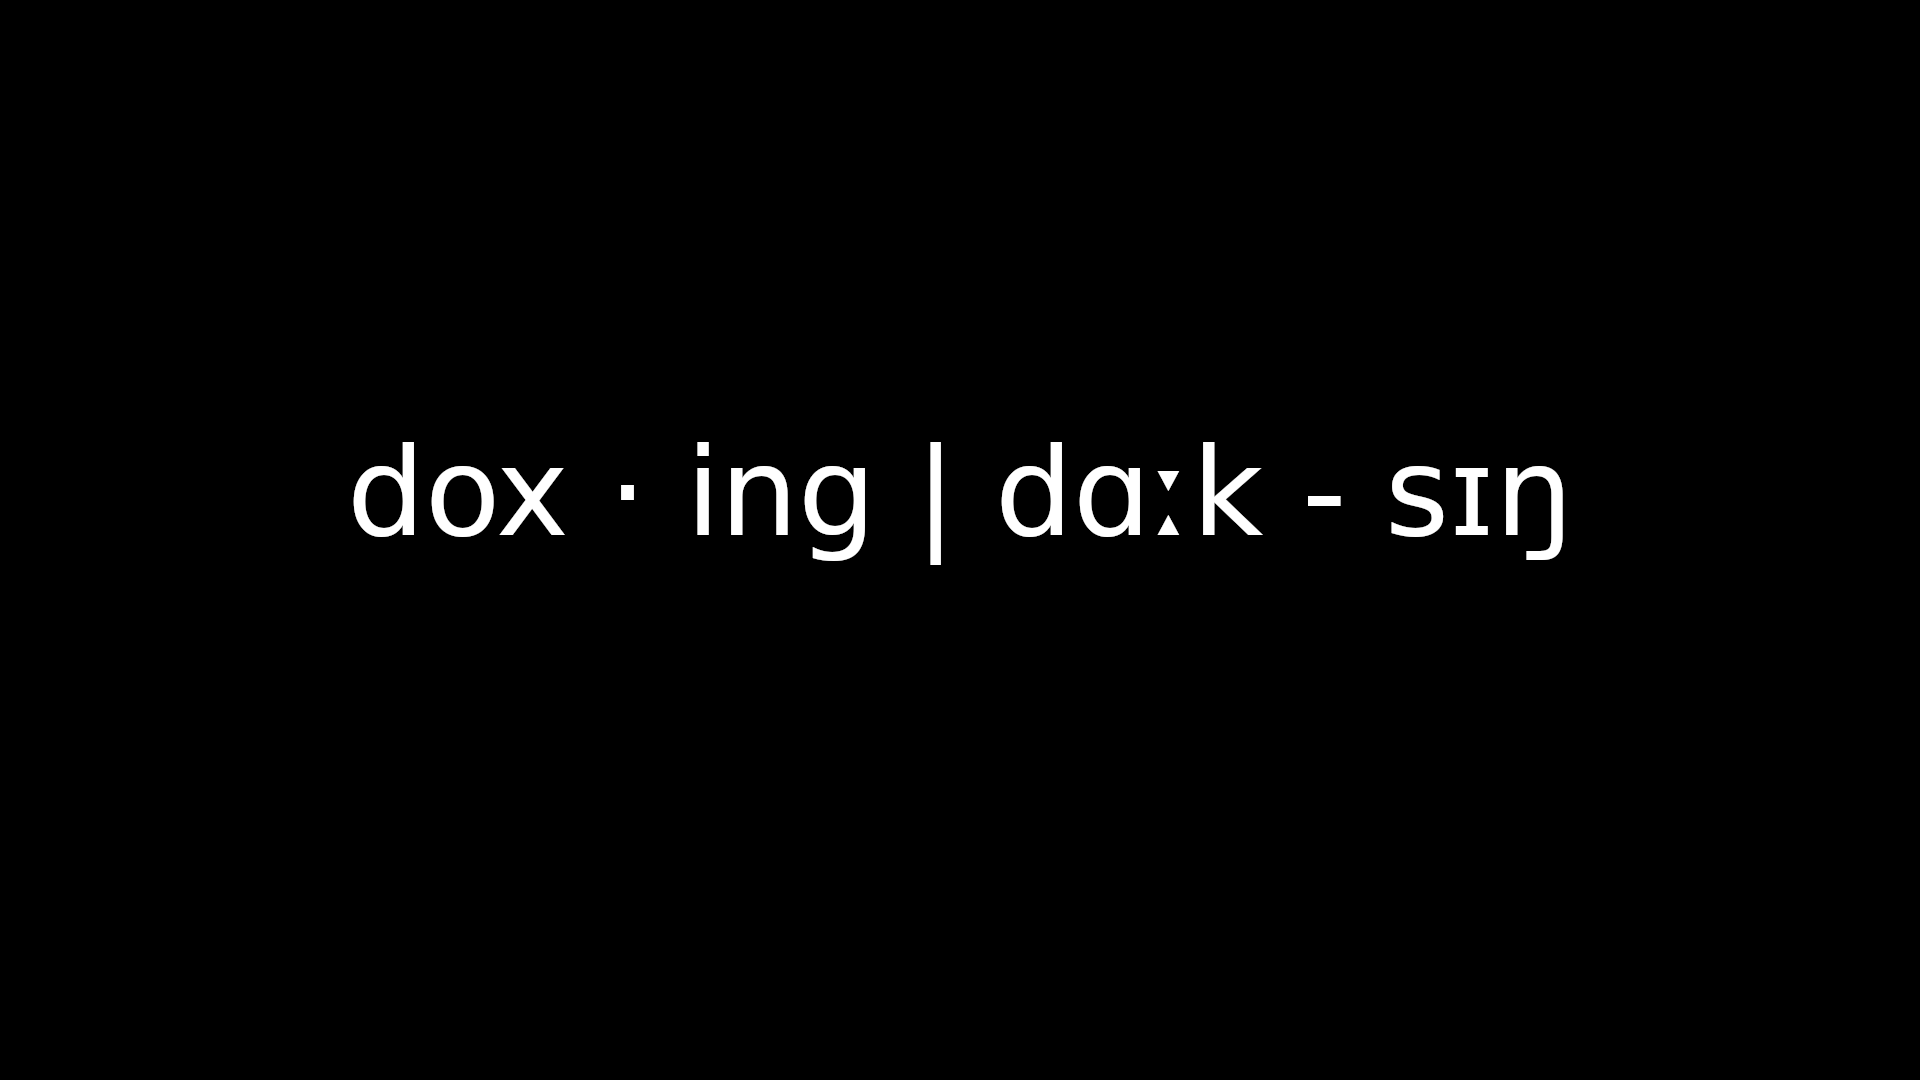
\includegraphics[width = \textwidth, height = .85\textheight, keepaspectratio]{figures/phonetics2.png} 

\end{colorframe}

\note{One possible escalation path is doxing. Or releasing personal information -such as name, address- of the victim online.

It is the step that brings online harrasment to real life and thus is a critical step in the escalation.
}



\begin{frame}
	\frametitle{Victims}
    
	\begin{itemize}
		\item Anyone
		\item Women
		\item Minorities
		\item LGBTQ
	\end{itemize}

\end{frame}

\note{While anyone can be the victim of cyberbullying, certain groups are at a disadvantage as it would appear internet's underbelly is full of trolls waiting for a chance to take a shot at those they consider easy prey.

Furthermore, certain threats are more impactful when directed to certain groups. Majority often does not have a traumatic history that they relate to these actions. The threat of sexual violence towards women, or slavery/genocide towards minorities can be more hurtful.}


\begin{frame}
	\frametitle{Beware}
    
    Oversharing \vspace{1em}

    Visibility \vspace{1em}

    Permanence \vspace{1em}

    Long Term Consequences

\end{frame}

\note{Before you share, think about these.

Once you share something online, there is no taking it back. Others will make copies, it will be archived, and saved beyond your control.

Treat everything you share as part of a permanent record. While you may be happy with your views now, in the long run you may regret it.

22\% of people in hiring positions report they have denied job applications based on social media history. }


{
\usebackgroundtemplate{
\includegraphics[width=\paperwidth,height=\paperheight]{internNoMore.png}}%
	\begin{frame}
	\frametitle{Exposure Online Brings Risks}



	\end{frame}
}

\note{It is hard to talk about real cases without re-victimizing the victim. }

\begin{frame}[t]
	\frametitle{Defence Against the Dark Arts}
	\framesubtitle{Is This The Hill You Want to Die on?}

	    \begin{columns}
			\begin{column}{0.6\textwidth}
	
				\vfill
				Do you really need the rest of humanity to know?
				\vfill
		
			\end{column}
	
			\begin{column}{0.3\textwidth}
	
				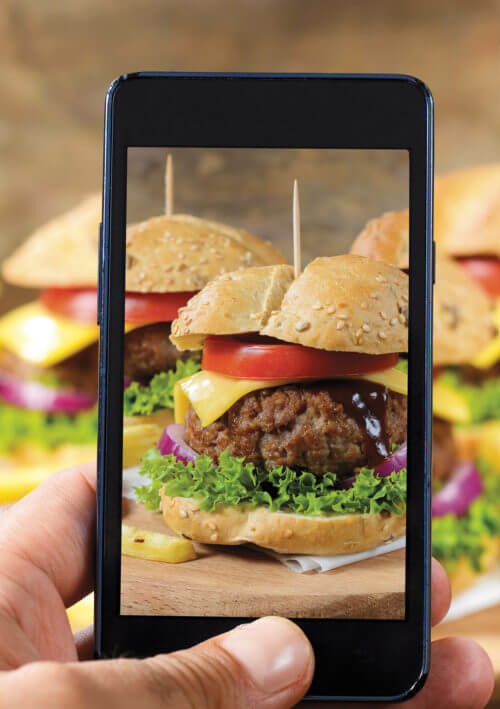
\includegraphics[width = \textwidth, height = \textheight, keepaspectratio]{figures/food.jpg}
	
			\end{column}
	
		\end{columns}
	


\end{frame}

\note{The point is not to discourage you from sharing your ideas online.

If you feel passionate about something, do go ahead.

Perhaps consider if you really need all 6.5 billion sweaty masses of us to know what you ate for lunch.}


\begin{frame}[t]
	\frametitle{Defence Against the Dark Arts}
	\framesubtitle{Who Can See What?}
	
	\centering
	\vfill
    \begin{tabular}{>{\centering\arraybackslash}m{3cm}ccc}
		\multicolumn{1}{c}{ } & \multicolumn{1}{c}{Profile} & \multicolumn{1}{c}{Posts} \\ \hline
		
\includegraphics[width = .1\textwidth, height = .1\textheight, keepaspectratio]{figures/Facebook.png}	& Public by Default		& Friends	\\
		
\includegraphics[width = .1\textwidth, height = .1\textheight, keepaspectratio]{figures/Instagram.png}	& Always Public			& Public	\\
		
\includegraphics[width = .1\textwidth, height = .1\textheight, keepaspectratio]{figures/Snapchat.png}	& Public by Default		& Friends	\\
		
\includegraphics[width = .1\textwidth, height = .1\textheight, keepaspectratio]{figures/Tiktok.png}		& Public by Default		& Public	\\
		
\includegraphics[width = .1\textwidth, height = .1\textheight, keepaspectratio]{figures/Twitter.png}	& Always Public			& Public	\\
	\end{tabular}	
	\vfill
\end{frame}

\note{}

\begin{frame}
	\frametitle{Privacy Settings}

	\centering
    
    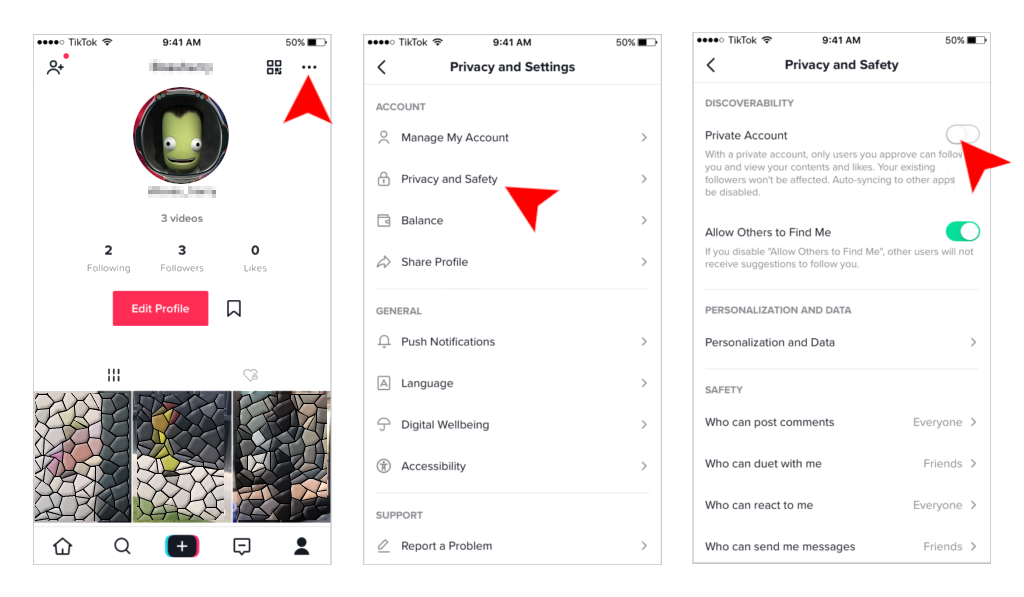
\includegraphics[width = \textwidth, height = .85\textheight, keepaspectratio]{figures/tik-tok-privacy-2-1024x597.png}

\end{frame}

\note{The least you can do is to make your account private.}


\begin{frame}
	\frametitle{Cyber Hygiene}
   
	\centering
	\vfill
	Password and Authentication Habbits 
	\vfill
\end{frame}

\note{While we will talk more about best practices for password and authentication mechanisms in a later module, it is worth noting here as well.

Reusing the same password, or not using MFA can enable attackers to expand their harrasment quickly.

To limit the damage, it is important to keep your accounts safe through MFA and strong passwords.}

\begin{frame}
	\frametitle{Recap}
    
    \begin{itemize}
    	\item Abuse and Harrassment Online
    	\item Factors Leading to Exposure
    	\item How to Respond
    \end{itemize}

\end{frame}

\note{Internet is a jungle. It can be beautiful but you need to watch out for yourself. Things you do online have consequences IRL.}

\end{document}
